\section{Evaluation}
    \label{sec:evaluation}
    \begin{figure*}
        \centering
        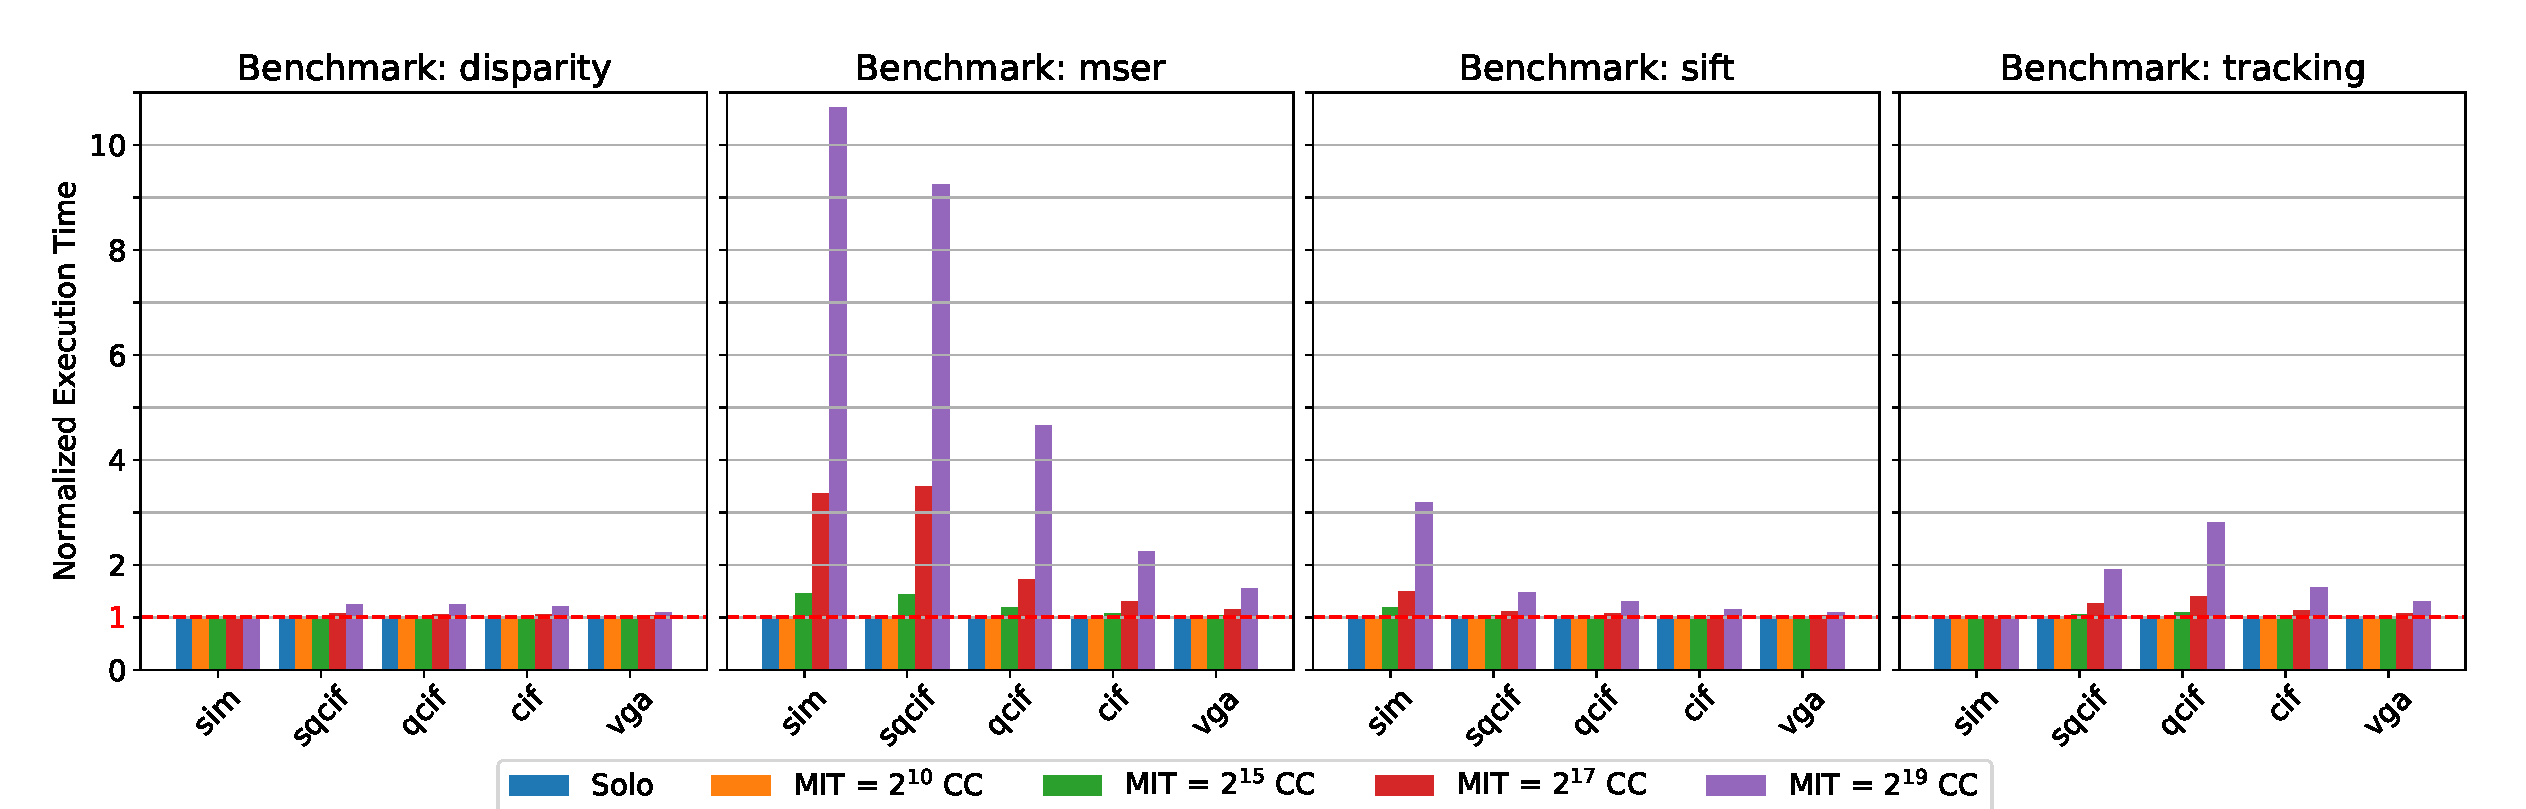
\includegraphics[scale=0.425]{images/cpu-brainfreeze-interference.pdf}
        \caption{Normailized execution time for different combinations of benchmark (inset), input sizes (x axis) and MITs (bar).}
        \label{fig:cpu-brainfreeze-interference-results}
    \end{figure*}

    For our experiment, we use the Xilinx ZCU102 development board \cite{Xilinx-ULTRASCALE-TRM}, a PS-PL platform featuring four ARM Cortex-A53 cores \cite{ARM-cortex-A53} connected together thanks to a shared LLC of 1MB.
    Thanks to the Jailhouse hypervisor \cite{jailhouse}, we are able to isolate the actors by assigning them specific cores and private partitions of the LLC.
    The victim inmate is allocated three cores and half of the LLC.
    It runs a selection of micro benchmarks issued from the San-Diego Vision Benchmark Suite \cite{SD-VBS} on top of Linux.
    The attacker is a lightweight baremetal inmate running on the remaining core.
    Finally, the PL side (and subsequently the AXI-Resistor) is clocked at 250MHz.\\

    Using the scenario and setup presented in section \ref{sec:system_model}, we aim at observing the interferences caused by the lightweight read attacker on the victim inmate.
    To this end, we run the selected set of micro benchmarks for all the available input sizes (x axis in Figure \ref{fig:cpu-brainfreeze-interference-results}) and different configurations of the AXI-Resistor (i.e. with MITs of $2^{10}$, $2^{15}$, $2^{17}$ and $2^{19}$).
    As a baseline, the benchmarks have also been run alone (i.e. without an attacker).
    This baseline is referred to as "Solo" in Figure \ref{fig:cpu-brainfreeze-interference-results}.
    All the results for the micro benchmarks (disparity, mser, sift and tracking) and its size input have been normalized with respect to the equivalent combination running alone (i.e. Solo, the leftmost blue bar in each bar cluster).

    From the results displayed in Figure \ref{fig:cpu-brainfreeze-interference-results}, two things can be observed.
    Firstly, the micro benchmarks have different sensitivity to the attacker. In fact, it is clear that the mser benchmark is more affected by the attacker than disparity.
    The former particularly suffers for a small input size (i.e. sim), with its execution time increased by a factor of 10.
    On the other hand, disparity seems unaffected by the attacker, meaning that spacial isolation of the core is enough.
    The increases of execution time observe in this experiment are in the same range as those reported by previous research.
    However, in our case, these interferences are caused by only one transaction instead of a continuous flow of transactions generated by 3 cores.
    Secondly, big MITs tend to introduce more inter-core interference than their counter part. For instance, a MIT of $2^{19}$ always introduce interference, regardless of its extent.\\

    Interrestingly, simulating an inifinite MIT by configuring the AXI-Resistor such that it would accept the transaction, but never answer systematically leads to the whole system being suspended indefinitely.
    In other words, if a task tries to fetch data from a memory that does not answer, not only its core stalls, but the whole core cluster is frozen.
    This suggest that for extremelly big MITs, important increase in execution could be observed and that all programs might be affected by the inter-core interference.
